\chapter{Nociones básicas}

Formalizamos algunas conceptos de probabilidad que vienen de la intuición. 


\section{Modelo probabilístico}

Consideremos un experimento con distintos posibles resultados. 

\begin{definition}
    El \emph{espacio muestral} de un experimento es el conjunto de posibles resultados del experimento. 
\end{definition}

Usualmente denotamos un espacio muestral con $\Omega$.

\begin{remark}
    Todo resultado corresponde con un único elemento $\omega \in \Omega$.
\end{remark}

Veamos algunos ejemplos.

\begin{example}
    \label{ex:dados}
    Consideremos el siguiente experimento:
    \begin{centeredvarwidth}
        \begin{enumerate}
            \item Se tira un dado balanceado de $6$ caras.
            \item Se graba el resultado.
        \end{enumerate}
    \end{centeredvarwidth}

    En este caso, el espacio muestral es el conjunto
    \begin{equation*}
        \Omega = \{ 1, 2, 3, 4, 5, 6 \}.
    \end{equation*}
\end{example}

Cabe aclarar que no importa de qué manera escribimos los resultados siempre y cuando la correspondencia con el resultado sea clara. Por ejemplo, podríamos haber definido el espacio muestral como
\begin{equation*}
    \Omega = \{ \vcdice{1}, \vcdice{2}, \vcdice{3}, \vcdice{4}, \vcdice{5}, \vcdice{6}\}.
\end{equation*}

\begin{example}
    Consideremos el siguiente experimento:
    \begin{centeredvarwidth}
        \begin{enumerate}
            \item Se tira una moneda $3$ veces.
            \item Se graba el resultado.
        \end{enumerate}
    \end{centeredvarwidth}

    El espacio muestral es
    \begin{equation*}
        \Omega = \{ CCC, CCS, \ldots, SSC, SSS \}.
    \end{equation*}
\end{example}

Nótese que $\Omega$ se puede escribir como $\{ C, S \}^3$.

\begin{example}
    Consideremos el siguiente experimento:
    \begin{centeredvarwidth}
        \begin{enumerate}
            \item Se elije un habitante de Buenos Aires al azar.
            \item Se mide su altura en metros.
        \end{enumerate}
    \end{centeredvarwidth}

    El espacio muestral podría ser
    \begin{equation*}
        \Omega = \R.
    \end{equation*}
\end{example}

Uno podría argumentar que el espacio muestral debería ser
\begin{equation*}
    \Omega = [0, 3],
\end{equation*}
ya que es imposible que alguien mida $\SI{-1}{m}$ o $\SI{100}{m}$. Sin embargo, lo único que nos interesa es que, al medir a alguien, caiga dentro de $\Omega$.


\section{Eventos}

\begin{definition}
    Sea $\Omega$ un espacio muestral. Un \emph{evento} es un subconjunto de $\Omega$.
\end{definition}

Veámoslo en algunos ejemplos.

\begin{example}
    Consideramos el experimento del ejemplo \ref{ex:dados}. El conjunto
    \begin{equation*}
        A = \{ \text{el resultado es un número par} \} = \{2, 4, 6\}
    \end{equation*}
    es un evento dado que $A \subseteq \Omega$.
\end{example}

Por ahora, usemos la noción intuitiva de probabilidades. 

La probabilidad se le asigna a un evento, no a un resultado. Por ejemplo, cuando decimos
\begin{equation*}
    P(\vcdice{3}) = \frac{1}{6}
\end{equation*}
en realidad queremos decir
\begin{equation*}
    P(\{ \vcdice{3} \}) = \frac{1}{6}.
\end{equation*}
No obstante, por practicidad acudiremos a la primera notación.

Usualmente calculamos la probabilidad de un evento de la siguiente manera:
\begin{equation*}
    P(A) = \frac{\# \text{ casos donde sucede } A}{\# \text{ casos totales}}.
\end{equation*}

Veamos por qué esto no es generalizable.

\begin{example}
    Consideremos el siguiente experimento:
    \begin{centeredvarwidth}
        \begin{enumerate}
            \item Se tiran $2$ dados balanceados de $6$ caras.
            \item Se suman los números de las caras.
            \item Se graba el resultado.
        \end{enumerate}
    \end{centeredvarwidth}

    Un espacio muestral podría ser
    \begin{equation*}
        \Omega = \{ 2, 3, \ldots, 12 \}.
    \end{equation*}
    Sin embargo, $P(2) \neq \frac{1}{10}$. Esto se puede resolver tomando el espacio muestral
    \begin{equation*}
        \Omega = \{ \vcdice{1} \vcdice{1}, \vcdice{1} \vcdice{2}, \ldots, \vcdice{6} \vcdice{5}, \vcdice{6} \vcdice{6} \}.
    \end{equation*}
    Por lo tanto, para todo resultado $\omega \in \Omega$, 
    \begin{equation*}
        P(\omega) = \frac{\# \text{ casos donde sucede } A}{\# \text{ casos totales}} = \frac{1}{36}.
    \end{equation*}
\end{example}

A partir de este ejemplo surge una definición.

\begin{definition}
    Sea $\Omega$ un espacio muestral. Si $\Omega$ es finito y todos sus elementos tienen la misma probabilidad, decimos que $\Omega$ es un \emph{espacio muestral equiprobable}.
\end{definition}

Sin embargo, hasta ahora únicamente tratamos con espacios muestrales finitos. Veamos qué pasa con los infinitos.

\begin{example}
    Consideremos el siguiente experimento:
    \begin{centeredvarwidth}
        \begin{enumerate}
            \item Se elije un punto del disco unitario $D = \{ (x, y) \in \R^2 \mid x^2 + y^2 = 1\}$ al azar.
            \item Se graba el resultado.
        \end{enumerate}
    \end{centeredvarwidth}

    Sea $A = \{ (x, y) \in \R^2 \mid x^2 + y^2 \leq \frac{1}{2} \}$.

    \begin{figure}[H]
        \centering
        \begin{tikzpicture}[scale=0.6]
            % Dibuja y rellena el círculo grande (espacio muestral Omega)
            \fill[black!10] (0,0) circle (3cm);
            \draw (0,0) circle (3cm);
            \node[above right] at (3,0) {$\Omega$};

            % Dibuja y rellena el círculo más pequeño (evento A)
            % Paso 1: Rellenar el círculo con un color sólido para el fondo
            \fill[primarycolor!20] (0,0) circle (2.1213cm);
            % Paso 2: Rellenar el mismo círculo con un patrón de líneas diagonales
            \fill[pattern=north east lines, pattern color=primarycolor!50] (0,0) circle (2.1213cm);
            % Borde del círculo A
            \draw[primarycolor, thick] (0,0) circle (2.1213cm);
            \node[below right] at (2,0) {$A$};
        \end{tikzpicture}
    \end{figure}

    Por lo que 
    \begin{equation*}
        P(A) = \frac{\area(A)}{\area(\Omega)}.
    \end{equation*}
\end{example}


\section{Eventos aleatorios}

No podemos definirle una probablidad a todos los eventos de un espacio muestral.

\begin{definition}
    Un evento al cual le podemos definir una probabilidad es llamado un \emph{evento aleatorios}.
\end{definition}

Agregamos algunas reglas adicionales.

\begin{definition}
    Llamamos $\mathcal{F}$ a una familia de eventos a los cuales podemos calcularles su probabilidad si cumple los siguientes axiomas:
    \begin{itemize}
        \item[(F1)] $\Omega \in \mathcal{F}$.
        \item[(F2)] Si $A \in \mathcal{F}$, entonces $A^{\textrm{c}} \in \mathcal{F}$.
        \item[(F3)] Si $\{A_n\}_{n \in \N} \subseteq \mathcal{F}$, entonces $\bigcup_{n \in \N} A_n \in \mathcal{F}$. 
    \end{itemize}
\end{definition}

\begin{remark}
    Si una familia cumple los axiomas (F1), (F2) y (F3), entonces se llama una $\sigma$-álgebra de conjuntos.
\end{remark}

\begin{example}
    En el ejemplo \ref{ex:dados}, el espacio muestral
    \begin{equation*}
        \Omega = \{ 1, 2, 3, 4, 5, 6 \}
    \end{equation*}
    tiene a la familia de eventos $\mathcal{F} = \mathcal{P}(\Omega)$ que se les puede asignar una probabilidad.
\end{example}

Veamos algunas propiedades que podemos deducir.

\begin{proposition}
    \label{prop:familia-eventos}
    Sea $\Omega$ un espacio muestral y $\mathcal{F} \subseteq \mathcal{P}(\Omega)$ una $\sigma$-álgebra. Las siguientes proposiciones son verdaderas:
    \begin{enumerate}
        \item $\varnothing \in \mathcal{F}$.
        \item Si $\{A_n\}_{1 \leq n \leq N} \subseteq \mathcal{F}$, entonces $\bigcup_{1 \leq n \leq N} A_n \in \mathcal{F}$.
        \item Si $\{A_n\}_{n \in \N} \subseteq \mathcal{F}$, entonces $\bigcap_{n \in \N} A_n \in \mathcal{F}$. (También la versión finita.)
        \item Si $A, B \in \mathcal{F}$, entonces $A \setminus B \in \mathcal{F}$.
    \end{enumerate}
\end{proposition}

\begin{proof}
    (\textit{1.}) Dado que $\Omega \in \mathcal{F}$ por (F1), obtenemos que $\varnothing = \Omega^{\textrm{c}} \in \mathcal{F}$ por (F2).

    (\textit{2.}) Sea $\{A_n\}_{1 \leq n \leq N} \subseteq \mathcal{F}$. Consideremos la familia $\{B_n\}_{n \in \N}$ tal que 
    \begin{equation*}
        B_n = \begin{cases}
            A_n & \text{si } 1 \leq n \leq N, \\
            \varnothing & \text{si } n \geq N. \\
        \end{cases}
    \end{equation*}
    Entonces, por (F3),
    \begin{equation*}
        \bigcup_{1 \leq n \leq N} A_n = \bigcup_{n \in \N} B_n \in \mathcal{F}.
    \end{equation*}

    (\textit{3.}) Sea $\{A_n\}_{n \in \N} \subseteq \mathcal{F}$. Por (F3),
    \begin{equation*}
        \bigcap_{n \in \N} A_n = \left(\bigcup_{n \in \N} A_n^{\mathrm{c}}\right)^{\textrm{c}} \in \mathcal{F}.
    \end{equation*}

    (\textit{4.}) Sean $A, B \in \mathcal{F}$. Dado que $B^{\mathrm{c}}$,
    \begin{equation*}
        A \setminus B = A \cap B^{\mathrm{c}} \in \mathcal{F}.
    \end{equation*}
\end{proof}

\begin{example}
    Consideremos el siguiente experimento:
    \begin{centeredvarwidth}
        \begin{enumerate}
            \item Se elije un número real del intervalo $[0, 1]$ al azar.
            \item Se graba el resultado.
        \end{enumerate}
    \end{centeredvarwidth}

    Sea $\Omega = [0, 1]$ el espacio muestral y sea $\mathcal{F}$ la familia de eventos a los cuales les podemos asignar una probabilidad. Para un intervalo $[a, b]$ la probabilidad se puede calcular como
    \begin{equation*}
        P([a, b]) = b - a.
    \end{equation*}

    Aplicando las propiedades de la proposición \ref{prop:familia-eventos}, podemos deducir que en $\mathcal{F}$ están los eventos:
    \begin{itemize}
        \item Los intervalos abiertos y cerrados.
        \item Uniones e intersecciones numerables de cerrados y/o abiertos.
        \item Los puntos $\{x\}$ con $x \in [0, 1]$.
        \item Los números racionales $\Q$.
    \end{itemize}

    ¿Cuál es la probabilidad de $\Q$? Basta con tomar $\{B_m\} = \{B(q_m, \frac{\varepsilon}{2^{m+1}})\}_{m \in \N}$ y ver que
    \begin{align*}
        P\left(\bigcup_{m \in \N} B_m\right) &\leq \sum_{m \in \N} P(B_m) \\
        &\leq \sum_{m \in \N} \frac{\varepsilon}{2^m} \\
        &\leq \varepsilon.
    \end{align*}
    Tomando $\varepsilon \to 0$, obtenemos que $P(\Q) = 0$.
\end{example}


\section{Definición de probabilidad}

La \textit{idea de Laplace} de probabilidad consta en que la probabilidad de un evento es el límite de la frecuencia con la que sucede cuando la cantidad de ensayos tiende a infinito.

Por otro lado, está la \textit{axiomatización de Kolmogorov}:

\begin{definition}
    Sea $\Omega$ un espacio muestra y $\mathcal{F} \subseteq \mathcal{P}(\Omega)$ una $\sigma$-álgebra. Una función probabilidad es una función $P: \mathcal{F} \to [0, 1]$ que cumple los siguientes axiomas:
    \begin{itemize}
        \item[(P1)] $P(\Omega) = 1$.
        \item[(P2)] $P(A) \geq 0$ para todo $A \in \mathcal{F}$.
        \item[(P3)] Si $\{A_n\}_{n \in \N} \subseteq \mathcal{F}$ una familia de eventos disjuntos, entonces $P(\bigcup_{n \in \N} A_n) = \sum_{n = 1}^{\infty} P(A_n)$.
    \end{itemize}
\end{definition}

Con esto podemos definir un espacio de probabilidad.

\begin{definition}
    Sea $\Omega$ un espacio muestral, $\mathcal{F} \subseteq \mathcal{P}(\Omega)$ una familia de eventos y $P: \mathcal{F} \to [0, 1]$ una función probabilidad. Entonces, la terna $(\Omega, \mathcal{F}, P)$ es un \emph{espacio de probabilidad}.
\end{definition}

%
% TODO: Propiedad de suma = 1 => terna espacio de proba
%

Probamos algunos resultados inmediatos.

\begin{proposition}
    Sea $(\Omega, \mathcal{F}, P)$ un espacio de probabilidad. Entonces, las siguientes proposiciones son verdaderas:
    \begin{enumerate}
        \item $P(\varnothing) = 0$.
        \item Si $A$ y $B$ son eventos disjuntos, entonces $P(A \cup B) = P(A) + P(B)$.
        \item Si $\{A_n\}_{1 \leq n \leq N}$ es una familia de eventos disjuntos, entonces $P(\bigcup_{1 \leq n \leq N} A_n) = \sum_{n = 1}^N P(A_n)$.
        \item $P(A^{\textrm{c}}) = 1 - P(A)$.
        \item Si $A \subseteq B$, entonces $P(A) \leq P(B)$.
        \item $P(\bigcup_{n \in \N} A_n) \leq \sum_{n = 1}^{\infty} P(A_n)$.
    \end{enumerate}
\end{proposition}

\begin{proof}
    (\textit{1.}) Consideremos la familia $\{ \Omega, \varnothing, \ldots \}$. Por (P3), 
    \begin{align*}
        P(\Omega) &= P(\Omega \cup \varnothing \cup \cdots) \\
        &= P(\Omega) + \underbrace{P(\varnothing) + \cdots}_{=0}
    \end{align*}

    (\textit{2.}) La propiedad sale utilizando (P3) y tomando la familia $\{ A, B, \varnothing, \ldots \}$.

    (\textit{3.}) Se prueba por inducción y ussando la proposición anterior.

    (\textit{4.}) Podemos escribir como unión disjunta $\Omega = A \cup A^{\mathrm{c}}$. Y con la propiedad \textit{2.} obtenemos que
    \begin{equation*}
        1 = P(\Omega) = P(A) + P(A^{\mathrm{c}}),
    \end{equation*}
    entonces
    \begin{equation*}
        P(A^{\mathrm{c}}) = 1 - P(A).
    \end{equation*}

    (\textit{5.}) Como $B = (B \setminus A) \cup A$,
    \begin{equation*}
        P(A) \leq P(B \setminus A) + P(A) = P(B).
    \end{equation*}

    (\textit{6.}) Sea $\{A_n\}_{n \in \N}$ una familia de eventos. Consideremos $\{B_n\}_{n \in \N}$ tal que
    \begin{equation*}
        B_n = A_n \setminus \bigcup_{1 \leq k \leq n-1} A_k.
    \end{equation*}
    Como los eventos $B_n$ son disjuntos dos a dos,
    \begin{equation*}
        P\left(\bigcup_{n \in \N} A_n\right) = P\left(\bigcup_{n \in \N} B_n\right) = \sum_{n = 1}^{\infty} P(B_n) \leq \sum_{n = 1}^{\infty} P(A_n).
    \end{equation*}
\end{proof}

\begin{example}
    \label{ex:moneda-hasta-cara}
    Consideremos el siguiente experimento:
    \begin{centeredvarwidth}
        \begin{enumerate}
            \item Se tira una moneda balanceada hasta que salga cara.
            \item Se anota la cantidad total de lanzamientos.
        \end{enumerate}
    \end{centeredvarwidth}

    El espacio muestral es
    \begin{equation*}
        \Omega = \N,
    \end{equation*}
    con
    \begin{equation*}
        P(1) = \frac{1}{2}, \quad P(i) = \frac{1}{2^i}, \quad i \geq 1.
    \end{equation*}
\end{example}

Ahora pensémoslo con infinitas tiradas de moneda.

\begin{example}
    Consideremos el experimento del ejemplo \ref{ex:moneda-hasta-cara}. Entonces, el espacio muestral es
    \begin{equation*}
        \Omega = \{0,1\}^{\N}.
    \end{equation*}

    Sea $C_k = \{ \text{la $k$-ésima moneda es cara} \}$ y definimos
    \begin{equation*}
        A_n = \{\text{las primeras $n$ monedas son cara}\}
        = \bigcap_{k=1}^n C_k.
    \end{equation*}
    Entonces, $P(A_n) = \frac{1}{2^n}$. Consideremos
    \begin{equation*}
        A = \{ \text{sale siempre cara} \} = \bigcap_{n \in \N} A_n.
    \end{equation*}
    Por lo tanto $A \subseteq A_n$ para todo $n \in \N$. Así, $P(A) \leq P(A_n) = \frac{1}{2^n} \to 0$ y $P(A) = 0$.

    Veamos otro evento:
    \begin{equation*}
        B = \{\text{a partir de algún momento salen sólo caras}\}.
    \end{equation*}
    Es decir, existe $n_0 \in \N$ tal que para todo $k \geq n_0$ la moneda $k$ es cara. En notación,
    \begin{equation*}
        B = \bigcup_{n_0 \in \N} \bigcap_{k=n_0}^\infty C_k.
    \end{equation*}

    Para cada $n_0$ fijo,
    \begin{align*}
        P\left(\bigcap_{k=n_0}^\infty C_k\right)
        &= \lim_{m \to \infty} P\left(\bigcap_{k=n_0}^m C_k\right) \\
        &= \lim_{m \to \infty} \frac{1}{2^{m-n_0+1}} \\
        &= 0.
    \end{align*}
    Entonces, por subaditividad numerable,
    \begin{equation*}
        P(B) \leq \sum_{n_0 \in \N} 0 = 0.
    \end{equation*}
\end{example}

Podemos mirar a $\omega = (\omega_k)_{k \in \N} \in \{0,1\}^\N$ como la expansión binaria de un número real $x \in [0,1]$:
\begin{equation*}
    x = \sum_{k=1}^\infty \frac{\omega_k}{2^k}.
\end{equation*}
De esta forma, elegir una secuencia infinita de lanzamientos es equivalente a elegir un número real en $[0,1]$.

\begin{figure}[H]
    \centering
    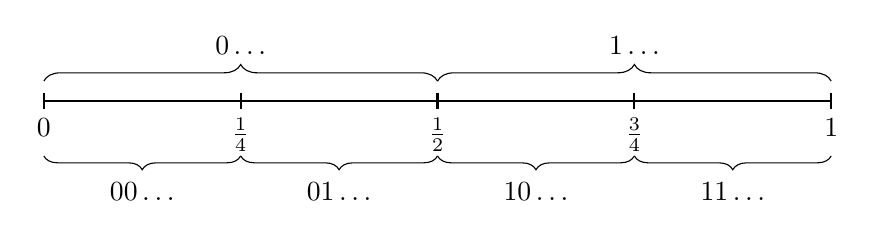
\begin{tikzpicture}[x=10cm,y=1cm]
        % segmento [0,1]
        \draw[thick] (0,0) -- (1,0);
        \foreach \x/\lab in {0/0,0.25/\frac14,0.5/\frac12,0.75/\frac34,1/1}{
            \draw[thick] (\x,0.1)--(\x,-0.1);
            \node[below] at (\x,-0.1) {$\lab$};
        }
        % llaves para 0/1
        \draw[decorate,decoration={brace,amplitude=6pt}] (0,0.25) -- (0.5,0.25) node[midway,above=6pt] {$0\ldots$};
        \draw[decorate,decoration={brace,amplitude=6pt}] (0.5,0.25) -- (1,0.25) node[midway,above=6pt] {$1\ldots$};
        % llaves para 00,01,10,11
        \draw[decorate,decoration={mirror,brace,amplitude=5pt}] (0,-0.7) -- (0.25,-0.7) node[midway,below=6pt] {$00\ldots$};
        \draw[decorate,decoration={mirror,brace,amplitude=5pt}] (0.25,-0.7) -- (0.5,-0.7) node[midway,below=6pt] {$01\ldots$};
        \draw[decorate,decoration={mirror,brace,amplitude=5pt}] (0.5,-0.7) -- (0.75,-0.7) node[midway,below=6pt] {$10\ldots$};
        \draw[decorate,decoration={mirror,brace,amplitude=5pt}] (0.75,-0.7) -- (1,-0.7) node[midway,below=6pt] {$11\ldots$};
    \end{tikzpicture}
\end{figure}

\begin{proposition}
    Sea $\{A_n\}_{n \in \N}$ una familia de eventos con $A_n \subseteq A_{n+1}$ para todo $n$. Entonces
    \begin{equation*}
        P\left(\bigcup_{n \in \N} A_n\right) = \lim_{n \to \infty} P(A_n).
    \end{equation*}
\end{proposition}

\begin{proof}
    Definimos $B_n = A_n \setminus A_{n-1}$ (con $A_0 = \varnothing$). Entonces
    \begin{equation*}
        \bigcup_{n \in \N} B_n = \bigcup_{n \in \N} A_n
        \qquad \text{y} \qquad
        B_i \cap B_j = \varnothing \;\; \text{si } i \neq j.
    \end{equation*}
    Como $P(B_n) = P(A_n) - P(A_{n-1})$, tenemos
    \begin{align*}
        P\left(\bigcup_{n \in \N} A_n\right)
        &= \sum_{n=1}^\infty P(B_n) \\
        &= \lim_{N \to \infty} \sum_{n=1}^N \big(P(A_n) - P(A_{n-1})\big) \\
        &= \lim_{N \to \infty} \big(P(A_N) - P(A_0)\big).
    \end{align*}
    Como $A_0 = \varnothing$, queda
    \begin{equation*}
        P\left(\bigcup_{n \in \N} A_n\right) = \lim_{N \to \infty} P(A_N).
    \end{equation*}
\end{proof}

\begin{corollary}
    Tomando complementos se obtiene que, si $A_n \supseteq A_{n+1}$, entonces
    \begin{equation*}
        P\left(\bigcap_{n \in \N} A_n\right)
        = 1 - P\left(\bigcup_{n \in \N} A_n^{\mathrm{c}}\right)
        = 1 - \lim_{n \to \infty} P(A_n^{\mathrm{c}})
        = \lim_{n \to \infty} P(A_n).
    \end{equation*}
\end{corollary}

\section{Probabilidad condicional}

Ya vimos cómo calcular probabilidades de eventos. Ahora queremos formalizar qué significa calcular probabilidades \textit{condicionadas} a que cierto evento ya ocurrió.

\begin{example}
    Tiro dos dados y sumo los resultados. Consideremos los eventos
    \begin{align*}
        A &= \{\text{la suma es $5$}\}, \\
        B &= \{\text{el segundo dado es par}\}.
    \end{align*}
    El espacio muestral es
    \begin{equation*}
        \Omega = \{(a,b) \mid a,b \in \{1,\ldots,6\}\}.
    \end{equation*}
    En particular,
    \begin{equation*}
        A = \{(1,4),(4,1),(2,3),(3,2)\}.
    \end{equation*}
    Luego,
    \begin{equation*}
        P(A \mid B) = \frac{\# (A \cap B)}{\# B} = \frac{2}{18} = \frac{1}{9}.
    \end{equation*}
\end{example}

El cálculo anterior nos motiva a introducir la definición general de probabilidad condicional.

\begin{definition}
    Dados $A$ y $B$ eventos, con $P(B) \neq 0$, la \emph{probabilidad condicional} de $A$ dado $B$ se define como
    \begin{equation*}
        P(A \mid B) = \frac{P(A \cap B)}{P(B)}.
    \end{equation*}
\end{definition}

Veamos cómo aplica la definición en un ejemplo.

\begin{example}
    Consideremos una urna con $9$ bolitas de la siguiente forma:
    \begin{itemize}
        \item $5$ naranjas,
        \item $4$ violetas, de las cuales $3$ tienen una cruz.
    \end{itemize}
    Denotemos $N=$ \{\text{naranja}\}, $V=$ \{\text{violeta}\}, $C=$ \{\text{tiene cruz}\}. Entonces,
    \begin{align*}
        P(N) &= \frac{5}{9}, &
        P(N \mid V) &= \frac{1}{3}, &
        P(C \mid V) &= \frac{1}{2}.
    \end{align*}
\end{example}

A partir de la definición, podemos verificar fácilmente que $P(\,\cdot \mid B)$ cumple los axiomas de probabilidad.

\begin{proposition}
    Sea $B$ un evento con $P(B) \neq 0$. Entonces la aplicación
    \begin{equation*}
        A \mapsto P(A \mid B)
    \end{equation*}
    define una probabilidad sobre el espacio muestral condicionado.
\end{proposition}

\begin{proof}
    Para todo $B$ con $P(B)>0$:
    \begin{itemize}
        \item[(P1)] $P(\Omega \mid B) = \frac{P(\Omega \cap B)}{P(B)} = \frac{P(B)}{P(B)}=1$.
        \item[(P2)] Como $P$ es una probabilidad, $P(A \mid B) \geq 0$.
        \item[(P3)] Si $\{A_n\}_{n \in \N}$ son eventos disjuntos dos a dos,
        \begin{align*}
            P\!\left(\bigcup_{n \in \N} A_n \,\middle|\, B\right)
            &= \frac{P\!\left(\bigcup_{n \in \N}(A_n \cap B)\right)}{P(B)} \\
            &= \frac{\sum_{n \in \N} P(A_n \cap B)}{P(B)} \\
            &= \sum_{n \in \N} \frac{P(A_n \cap B)}{P(B)} \\
            &= \sum_{n \in \N} P(A_n \mid B).
        \end{align*}
    \end{itemize}
\end{proof}

\begin{remark}
    Es importante aclarar que $A \mid B$ no es un evento. Por lo tanto, expresiones como $P(A \mid B \mid C)$ no tienen sentido.
\end{remark}

\begin{proposition}
    Para todo par de eventos $A, B$ con $P(B) \neq 0$, se cumple
    \begin{equation*}
        P(A \mid B) \, P(B) = P(A \cap B).
    \end{equation*}
\end{proposition}

Este resultado es útil para calcular probabilidades conjuntas a partir de probabilidades condicionales.

\begin{example}
    Sacamos dos cartas de un mazo de $52$ cartas sin reemplazo. Sea
    \begin{align*}
        A_1 &= \{\text{la primera carta es trébol}\}, \\
        A_2 &= \{\text{la segunda carta es trébol}\}.
    \end{align*}
    Entonces,
    \begin{align*}
        P(A_1) &= \frac{13}{52}, \\
        P(A_2 \mid A_1) &= \frac{12}{51}.
    \end{align*}
    Aplicando la proposición anterior,
    \begin{equation*}
        P(A_1 \cap A_2) = P(A_1)\,P(A_2 \mid A_1) = \frac{13}{52} \cdot \frac{12}{51}.
    \end{equation*}
\end{example}

\begin{proposition}[Regla del producto]
    Para eventos $A_1, A_2, \dots, A_n$ se cumple
    \begin{equation*}
        P(A_1 \cap A_2 \cap \cdots \cap A_n)
        = P(A_1)\,P(A_2 \mid A_1)\,P(A_3 \mid A_1 \cap A_2)\,\cdots\,P(A_n \mid A_1 \cap \cdots \cap A_{n-1}).
    \end{equation*}
\end{proposition}

\begin{proof}[Idea de demostración]
    La demostración se hace fácilmente por inducción en $n$.
\end{proof}

\section{Probabilidad total}

La noción de probabilidad condicional nos permite descomponer probabilidades en términos de eventos disjuntos.

\begin{proposition}[Probabilidad total en dos partes]
    Sea $B \subseteq \Omega$ un evento. Entonces, para todo $A \subseteq \Omega$,
    \begin{align*}
        P(A) &= P(A \cap B) + P(A \cap B^{\mathrm c}) \\
             &= P(A \mid B)\,P(B) + P(A \mid B^{\mathrm c})\,P(B^{\mathrm c}).
    \end{align*}
\end{proposition}

Más en general, si $\{A_i\}_{i \in I}$ es una partición numerable de $\Omega$, se cumple la \textit{ley de la probabilidad total}:
\begin{equation*}
    P(B) = \sum_{i \in I} P(B \mid A_i)\,P(A_i).
\end{equation*}

\begin{example}
    Consideremos el siguiente experimento:
    \begin{centeredvarwidth}
        \begin{enumerate}
            \item En una caja hay $3$ monedas: una con dos caras y dos equilibradas.
            \item Se elige una moneda al azar.
            \item Se lanza la moneda.
        \end{enumerate}
    \end{centeredvarwidth}

    Definamos los eventos
    \begin{align*}
        C &= \{\text{sale cara}\}, \\
        A &= \{\text{la moneda elegida es la de dos caras}\}.
    \end{align*}

    Entonces,
    \begin{align*}
        P(C) &= P(C \mid A)\,P(A) + P(C \mid A^{\mathrm{c}})\,P(A^{\mathrm{c}}) \\
             &= 1 \cdot \frac{1}{3} + \frac{1}{2} \cdot \frac{2}{3} \\
             &= \frac{2}{3}.
    \end{align*}
\end{example}

Este cálculo es un primer ejemplo de la \emph{fórmula de la probabilidad total}, que nos permite descomponer la probabilidad de un evento en función de una partición del espacio.

\begin{example}
    Ahora consideremos otro experimento. Lanzamos un dado. Sea
    \begin{align*}
        A &= \{\text{saco un $5$}\}, \\
        B &= \{\text{saco un $7$}\}, \\
        C &= \{\text{ni $5$ ni $7$}\} = (A \cup B)^{\mathrm c}.
    \end{align*}

    Supongamos que ganar depende de estos eventos: 
    si ocurre $A$ se gana siempre, 
    si ocurre $B$ nunca se gana, 
    y si ocurre $C$ se gana con cierta probabilidad.

    Denotemos $G=\{\text{ganar}\}$. Entonces, por probabilidad total,
    \begin{align*}
        P(G) &= P(G \mid A)\,P(A) + P(G \mid B)\,P(B) + P(G \mid C)\,P(C).
    \end{align*}

    Como $P(G \mid A)=1$, $P(G \mid B)=0$, y $P(A)=P(B)=\frac{1}{6}$, $P(C)=\frac{4}{6}$, se obtiene
    \begin{align*}
        P(G) &= 1 \cdot \frac{1}{6} + 0 \cdot \frac{1}{6} + P(G \mid C)\,\frac{4}{6}.
    \end{align*}

    Si además sabemos que $P(G \mid C)=\frac{1}{2}$, queda
    \begin{equation*}
        P(G) = \frac{1}{6} + \frac{1}{2}\cdot\frac{4}{6} = \frac{6}{15}.
    \end{equation*}
\end{example}

Estos ejemplos muestran cómo las probabilidades condicionales y la probabilidad total se combinan para calcular probabilidades en situaciones más complejas.
